% Practice Test 02 — Indiana Edition
% Questions: 30 (22 MC + 8 SA)
% Generated by scripts/generate_practice_tests.py

\begin{practiceQuestion}{1-3-q30}{gsa}
\begin{questionText}
The table shows a proportional relationship between minutes and laps completed. Find $k$ and determine how many laps are completed in $15$ minutes.

\begin{center}
\begin{tabular}{|c|c|}
\hline
\textbf{Minutes ($x$)} & \textbf{Laps ($y$)} \\ \hline
$4$ & $3$ \\ \hline
$8$ & $6$ \\ \hline
$12$ & $9$ \\ \hline
$15$ & $?$ \\ \hline
\end{tabular}
\end{center}
\end{questionText}
\correctAnswer{$k = 0.75$; $11.25$ laps in $15$ minutes}
\explanation{$k = \frac{3}{4} = 0.75$. For $15$ minutes: $y = 0.75 \times 15 = 11.25$ laps.}
\end{practiceQuestion}

\begin{practiceQuestion}{1-5-q07}{mc}
\begin{questionText}
A line passes through $(0, 0)$ and has a slope of $\frac{3}{4}$. What is the $y$-value when $x = 8$?
\end{questionText}
\choiceA{$3$}
\choiceB{$6$}
\choiceC{$8$}
\choiceD{$11$}
\correctAnswer{B}
\explanation{$y = \frac{3}{4} \times 8 = 6$.}
\end{practiceQuestion}

\begin{practiceQuestion}{1-6-q25}{sa}
\begin{questionText}
A truck delivers $540$ packages in $3$ trips. How many trips are needed to deliver $1{,}620$ packages?
\end{questionText}
\correctAnswer{$9$ trips}
\explanation{Per trip: $540 \div 3 = 180$ packages. Trips needed: $1{,}620 \div 180 = 9$.}
\end{practiceQuestion}

\begin{practiceQuestion}{2-2-q13}{mc}
\begin{questionText}
A town has $2{,}400$ households. A survey shows $78\%$ have internet access. How many households have internet?
\end{questionText}
\choiceA{$1{,}800$}
\choiceB{$1{,}848$}
\choiceC{$1{,}872$}
\choiceD{$1{,}920$}
\correctAnswer{C}
\explanation{$\frac{n}{2400} = \frac{78}{100}$. Cross-multiply: $100n = 187{,}200$. Divide: $n = 1{,}872$.}
\end{practiceQuestion}

\begin{practiceQuestion}{2-5-q06}{mc}
\begin{questionText}
A taxi ride costs $\$18$. You tip the driver $18\%$. What is the total you pay?
\end{questionText}
\choiceA{$\$3.24$}
\choiceB{$\$19.80$}
\choiceC{$\$21.24$}
\choiceD{$\$21.60$}
\correctAnswer{C}
\explanation{Tip: $18 \times 0.18 = \$3.24$. Total: $18 + 3.24 = \$21.24$.}
\end{practiceQuestion}

\begin{practiceQuestion}{2-7-q10}{mc}
\begin{questionText}
A weather forecast predicted $3$ inches of rain. The actual rainfall was $2.5$ inches. What is the percent error?
\end{questionText}
\choiceA{$0.5\%$}
\choiceB{$10\%$}
\choiceC{$16.7\%$}
\choiceD{$20\%$}
\correctAnswer{D}
\explanation{$\frac{|3 - 2.5|}{2.5} \times 100 = \frac{0.5}{2.5} \times 100 = 20\%$.}
\end{practiceQuestion}

\begin{practiceQuestion}{3-1-q30}{gsa}
\begin{questionText}
A vertical number line shows the elevations of four locations.

\begin{center}
\begin{tikzpicture}
  \draw[thick,->] (0,-3.5) -- (0,4.5);
  \foreach \y in {-3,...,4} \draw (-0.15,\y) -- (0.15,\y) node[right=4pt] {$\y 00$ ft};
  \fill[funBlue] (0,3) circle (4pt) node[left=8pt] {Mountain};
  \fill[funGreen] (0,1) circle (4pt) node[left=8pt] {Hill};
  \fill[funOrange] (0,0) circle (4pt) node[left=8pt] {Beach};
  \fill[funRed] (0,-2) circle (4pt) node[left=8pt] {Valley};
  \draw[dashed,gray] (-0.5,0) -- (0.5,0);
  \node[right=20pt] at (0,0) {Sea Level};
\end{tikzpicture}
\end{center}

What is the difference in elevation between the Mountain and the Valley?
\end{questionText}
\correctAnswer{$500$ ft}
\explanation{Mountain is at $300$ ft and Valley is at $-200$ ft. Difference $= 300 - (-200) = 300 + 200 = 500$ ft.}
\end{practiceQuestion}

\begin{practiceQuestion}{3-2-q01}{mc}
\begin{questionText}
What is $(-8) + (-5)$?
\end{questionText}
\choiceA{$13$}
\choiceB{$-13$}
\choiceC{$-3$}
\choiceD{$3$}
\correctAnswer{B}
\explanation{Same signs: add the absolute values $8 + 5 = 13$ and keep the negative sign: $-13$.}
\end{practiceQuestion}

\begin{practiceQuestion}{4-2-q23}{sa}
\begin{questionText}
The perimeter of a triangle is $3x + 2 + 5x - 1 + 2x + 4$. Write the simplified expression for the perimeter.
\end{questionText}
\correctAnswer{$10x + 5$}
\explanation{Combine variable terms: $3x + 5x + 2x = 10x$. Combine constants: $2 - 1 + 4 = 5$. Perimeter: $10x + 5$.}
\end{practiceQuestion}

\begin{practiceQuestion}{4-3-q15}{mc}
\begin{questionText}
Expand $-5(x + 2)$.
\end{questionText}
\choiceA{$-5x + 10$}
\choiceB{$-5x + 2$}
\choiceC{$-5x - 10$}
\choiceD{$5x - 10$}
\correctAnswer{C}
\explanation{$-5 \times x = -5x$ and $-5 \times 2 = -10$. Result: $-5x - 10$.}
\end{practiceQuestion}

\begin{practiceQuestion}{5-4-q21}{sa}
\begin{questionText}
Solve $\dfrac{x}{2} + \dfrac{x}{4} = 9$.
\end{questionText}
\correctAnswer{$x = 12$}
\explanation{Multiply every term by $4$: $2x + x = 36$. Combine: $3x = 36$. Divide by $3$: $x = 12$. Check: $\frac{12}{2} + \frac{12}{4} = 6 + 3 = 9$ \checkmark.}
\end{practiceQuestion}

\begin{practiceQuestion}{5-5-q05}{mc}
\begin{questionText}
When do you flip the inequality sign?
\end{questionText}
\choiceA{When you add a negative number to both sides}
\choiceB{When you subtract from both sides}
\choiceC{When you multiply or divide both sides by a negative number}
\choiceD{When the variable is on the right side}
\correctAnswer{C}
\explanation{The inequality sign flips only when you multiply or divide both sides by a negative number.}
\end{practiceQuestion}

\begin{practiceQuestion}{5-6-q09}{mc}
\begin{questionText}
A parking garage charges $\$5$ per hour. You have $\$30$. Which inequality represents the hours $h$ you can park, and what does the graph look like?
\end{questionText}
\choiceA{$5h \leq 30$; closed circle at $6$, shade left from $0$ to $6$}
\choiceB{$5h < 30$; open circle at $6$, shade left}
\choiceC{$5h \geq 30$; closed circle at $6$, shade right}
\choiceD{$5h > 30$; open circle at $6$, shade right}
\correctAnswer{A}
\explanation{You can spend at most $\$30$: $5h \leq 30$, so $h \leq 6$. Closed circle at $6$, shade left (and $h \geq 0$).}
\end{practiceQuestion}

\begin{practiceQuestion}{6-1-q12}{mc}
\begin{questionText}
A scale drawing of a garden uses $1$ in $= 5$ ft. The drawing shows a square garden with side length $3$ in. What is the actual area of the garden?
\end{questionText}
\choiceA{$9$ ft$^2$}
\choiceB{$15$ ft$^2$}
\choiceC{$45$ ft$^2$}
\choiceD{$225$ ft$^2$}
\correctAnswer{D}
\explanation{Actual side: $3 \times 5 = 15$ ft. Actual area: $15 \times 15 = 225$ ft$^2$.}
\end{practiceQuestion}

\begin{practiceQuestion}{6-3-q04}{mc}
\begin{questionText}
You know two sides of a triangle are $7$ cm and $10$ cm, and the angle between them is $45°$. How many different triangles can you draw?
\end{questionText}
\choiceA{None}
\choiceB{Exactly one}
\choiceC{Exactly two}
\choiceD{Infinitely many}
\correctAnswer{B}
\explanation{Two sides and the included angle (SAS) fully determine one unique triangle.}
\end{practiceQuestion}

\begin{practiceQuestion}{6-4-q16}{mc}
\begin{questionText}
Which set of measurements does NOT determine a unique triangle?
\end{questionText}
\choiceA{Sides $3$, $4$, $5$}
\choiceB{Sides $7$ and $9$ with included angle $50°$}
\choiceC{Angles $40°$, $70°$, $70°$}
\choiceD{Angles $30°$, $60°$ with included side $10$ cm}
\correctAnswer{C}
\explanation{AAA alone does not fix the size of the triangle. Many triangles can share these angle measures.}
\end{practiceQuestion}

\begin{practiceQuestion}{6-5-q26}{gmc}
\begin{questionText}
The diagram shows a rectangular prism being sliced by a horizontal plane (dashed line). What is the cross-section?

\begin{center}
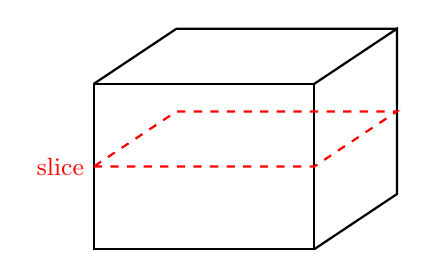
\begin{tikzpicture}[scale=0.7]
  % Rectangular prism
  \draw[thick] (0,0) -- (4,0) -- (4,3) -- (0,3) -- cycle; % front face
  \draw[thick] (4,0) -- (5.5,1) -- (5.5,4) -- (4,3); % right face
  \draw[thick] (0,3) -- (1.5,4) -- (5.5,4); % top face
  \draw[dashed,thick,red] (0,1.5) -- (4,1.5) -- (5.5,2.5) -- (1.5,2.5) -- cycle;
  \node[left,red] at (0,1.5) {\small slice};
\end{tikzpicture}
\end{center}
\end{questionText}
\choiceA{Triangle}
\choiceB{Rectangle}
\choiceC{Circle}
\choiceD{Trapezoid}
\correctAnswer{B}
\explanation{A horizontal slice through a rectangular prism always produces a rectangle congruent to the base.}
\end{practiceQuestion}

\begin{practiceQuestion}{6-6-q07}{mc}
\begin{questionText}
Two vertical angles are $(5x - 20)°$ and $(3x + 10)°$. What is the measure of each angle?
\end{questionText}
\choiceA{$45°$}
\choiceB{$55°$}
\choiceC{$60°$}
\choiceD{$75°$}
\correctAnswer{B}
\explanation{Vertical angles are equal: $5x - 20 = 3x + 10$. Subtract $3x$: $2x - 20 = 10$. Add $20$: $2x = 30$. Divide: $x = 15$. Angle: $5(15) - 20 = 55°$.}
\end{practiceQuestion}

\begin{practiceQuestion}{6-7-q28}{gmc}
\begin{questionText}
The coordinate plane shows point $U$ and its image $U'$ after a reflection. Over which axis was $U$ reflected?

\begin{center}
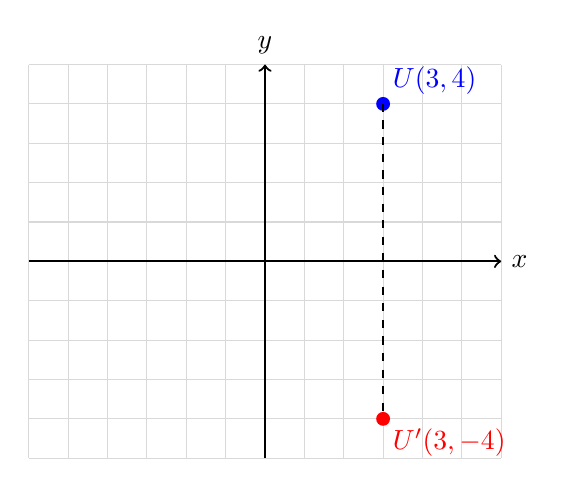
\begin{tikzpicture}[scale=0.5]
  \draw[step=1,gray!30,thin] (-6,-5) grid (6,5);
  \draw[thick,->] (-6,0) -- (6,0) node[right]{$x$};
  \draw[thick,->] (0,-5) -- (0,5) node[above]{$y$};
  \fill[blue] (3,4) circle (5pt);
  \node[above right,blue] at (3,4) {$U(3,4)$};
  \fill[red] (3,-4) circle (5pt);
  \node[below right,red] at (3,-4) {$U'(3,-4)$};
  \draw[dashed,thick] (3,4) -- (3,-4);
\end{tikzpicture}
\end{center}
\end{questionText}
\choiceA{The $x$-axis}
\choiceB{The $y$-axis}
\choiceC{The line $y = x$}
\choiceD{The line $x = 3$}
\correctAnswer{A}
\explanation{The $x$-coordinate stayed the same ($3$) and the $y$-coordinate changed sign ($4 \to -4$). This is a reflection over the $x$-axis.}
\end{practiceQuestion}

\begin{practiceQuestion}{7-3-q29}{gsa}
\begin{questionText}
The diagram shows a circular swimming pool. Find the area of the pool. Use $\pi \approx 3.14$.

\begin{center}
\begin{tikzpicture}[scale=0.4]
  \fill[cyan!20] (0,0) circle (3.5);
  \draw[thick,funBlue] (0,0) circle (3.5);
  \fill (0,0) circle (2pt) node[below] {center};
  \draw[thick,funRed,<->] (-3.5,0) -- (3.5,0);
  \node[above,funRed] at (0,0.2) {$18$ m};
\end{tikzpicture}
\end{center}
\end{questionText}
\correctAnswer{$254.34$ m$^2$}
\explanation{$r = 18 \div 2 = 9$ m. $A = \pi r^2 = 3.14 \times 81 = 254.34$ m$^2$.}
\end{practiceQuestion}

\begin{practiceQuestion}{7-4-q12}{mc}
\begin{questionText}
A square has sides of $10$ m. A quarter circle with radius $10$ m is removed from one corner. What is the area of the remaining figure? Use $\pi \approx 3.14$.
\end{questionText}
\choiceA{$21.5$ m$^2$}
\choiceB{$50$ m$^2$}
\choiceC{$78.5$ m$^2$}
\choiceD{$100$ m$^2$}
\correctAnswer{A}
\explanation{Square: $100$ m$^2$. Quarter circle: $\frac{1}{4} \times 3.14 \times 100 = 78.5$ m$^2$. Remaining: $100 - 78.5 = 21.5$ m$^2$.}
\end{practiceQuestion}

\begin{practiceQuestion}{7-5-q28}{gmc}
\begin{questionText}
The diagram shows a triangular prism. What is its total surface area?

\begin{center}
\begin{tikzpicture}[scale=0.4]
  % Front triangle
  \draw[thick,funBlue,fill=funBlue!10] (0,0) -- (6,0) -- (3,4) -- cycle;
  % Back triangle (offset)
  \draw[thick,funBlue,fill=funBlue!20] (2,1.5) -- (8,1.5) -- (5,5.5) -- cycle;
  % Connecting edges
  \draw[thick,funBlue] (0,0) -- (2,1.5);
  \draw[thick,funBlue] (6,0) -- (8,1.5);
  \draw[thick,funBlue] (3,4) -- (5,5.5);
  % Labels
  \node[below] at (3,0) {$6$ cm};
  \node[left] at (1.2,2) {$5$ cm};
  \node[right] at (4.8,2) {$5$ cm};
  \node[right] at (8,3.5) {$8$ cm};
  \node[above left] at (1,0.8) {$h = 4$ cm};
\end{tikzpicture}
\end{center}
\end{questionText}
\choiceA{$104$ cm$^2$}
\choiceB{$128$ cm$^2$}
\choiceC{$152$ cm$^2$}
\choiceD{$160$ cm$^2$}
\correctAnswer{C}
\explanation{Two triangles: $2 \times \frac{1}{2} \times 6 \times 4 = 24$ cm$^2$. Three rectangles: $6 \times 8 + 5 \times 8 + 5 \times 8 = 48 + 40 + 40 = 128$ cm$^2$. Total: $24 + 128 = 152$ cm$^2$.}
\end{practiceQuestion}

\begin{practiceQuestion}{7-6-q13}{mc}
\begin{questionText}
If you triple the height of a rectangular prism while keeping the base the same, what happens to the volume?
\end{questionText}
\choiceA{It stays the same}
\choiceB{It doubles}
\choiceC{It triples}
\choiceD{It increases by a factor of $9$}
\correctAnswer{C}
\explanation{$V = Bh$. If $h$ becomes $3h$, then $V = B(3h) = 3Bh$. The volume triples.}
\end{practiceQuestion}

\begin{practiceQuestion}{8-1-q10}{mc}
\begin{questionText}
Which question would require sampling rather than surveying the entire population?
\end{questionText}
\choiceA{How many students are in a classroom of $25$?}
\choiceB{What is the average lifespan of a light bulb produced by a factory?}
\choiceC{What is the total number of books on a shelf?}
\choiceD{How many chairs are in a room?}
\correctAnswer{B}
\explanation{Testing every light bulb would destroy them all. Sampling lets you estimate the average without testing every one.}
\end{practiceQuestion}

\begin{practiceQuestion}{8-3-q08}{mc}
\begin{questionText}
The dot plots for two classes overlap significantly. The difference in their means is $2$ points, and both have a MAD of $6$. What can you conclude?
\end{questionText}
\choiceA{The classes are very different}
\choiceB{The difference in means is meaningful}
\choiceC{The difference in means is small relative to the variability}
\choiceD{You cannot compare the classes}
\correctAnswer{C}
\explanation{The difference ($2$) is much smaller than the MAD ($6$), so the difference is not very meaningful — there is a lot of overlap.}
\end{practiceQuestion}

\begin{practiceQuestion}{8-4-q06}{mc}
\begin{questionText}
Team X: mean $82$, MAD $5$. Team Y: mean $76$, MAD $5$. Which team performed better on average, and is the difference meaningful?
\end{questionText}
\choiceA{Team X; no, because the difference is less than $2$ MADs}
\choiceB{Team X; yes, because $\frac{6}{5} = 1.2$ MADs, which is meaningful}
\choiceC{Team X; yes, because the means are more than $2$ MADs apart}
\choiceD{Team Y; yes, because its MAD is the same}
\correctAnswer{A}
\explanation{Difference $= 82 - 76 = 6$. In MADs: $\frac{6}{5} = 1.2$. Since $1.2 < 2$, the difference is not considered very meaningful.}
\end{practiceQuestion}

\begin{practiceQuestion}{8-7-q29}{gsa}
\begin{questionText}
The double bar graph compares test scores for two classes over three tests.

\begin{center}
\begin{tikzpicture}[scale=0.5]
  \draw[thick,->] (0,0) -- (0,6.5) node[above]{\small Average Score};
  \draw[thick,->] (0,0) -- (8.5,0);
  % Test 1
  \fill[funBlue!70] (0.5,0) rectangle (1.5,4);
  \fill[funOrange!70] (1.6,0) rectangle (2.6,3.5);
  \node[below,font=\tiny] at (1.55,0) {Test 1};
  % Test 2
  \fill[funBlue!70] (3.2,0) rectangle (4.2,4.5);
  \fill[funOrange!70] (4.3,0) rectangle (5.3,5);
  \node[below,font=\tiny] at (4.25,0) {Test 2};
  % Test 3
  \fill[funBlue!70] (5.9,0) rectangle (6.9,5);
  \fill[funOrange!70] (7.0,0) rectangle (8.0,4);
  \node[below,font=\tiny] at (6.95,0) {Test 3};
  \foreach \y in {1,...,6} { \draw (-0.1,\y) -- (0.1,\y); \node[left,font=\tiny] at (0,\y) {$\y\times 15$}; }
  \node[above,font=\tiny] at (1,4) {$60$};
  \node[above,font=\tiny] at (2.1,3.5) {$52$};
  \node[above,font=\tiny] at (3.7,4.5) {$68$};
  \node[above,font=\tiny] at (4.8,5) {$75$};
  \node[above,font=\tiny] at (6.4,5) {$75$};
  \node[above,font=\tiny] at (7.5,4) {$60$};
\end{tikzpicture}
\end{center}

Class A (blue): $60, 68, 75$. Class B (orange): $52, 75, 60$. Find the mean for each class. Which class improved more consistently?
\end{questionText}
\correctAnswer{Class A mean $\approx 67.7$; Class B mean $= 62.3$. Class A improved consistently (scores went up each test).}
\explanation{Class A: $\frac{60+68+75}{3} = \frac{203}{3} \approx 67.7$. Class B: $\frac{52+75+60}{3} = \frac{187}{3} \approx 62.3$. Class A's scores increased each test; Class B went up then down.}
\end{practiceQuestion}

\begin{practiceQuestion}{9-4-q13}{mc}
\begin{questionText}
A probability model has outcomes A, B, and C with $P(A) = 0.5$ and $P(B) = 0.3$. What is $P(C)$?
\end{questionText}
\choiceA{$0.8$}
\choiceB{$0.3$}
\choiceC{$0.2$}
\choiceD{$0.1$}
\correctAnswer{C}
\explanation{All probabilities must sum to $1$. $P(C) = 1 - 0.5 - 0.3 = 0.2$.}
\end{practiceQuestion}

\begin{practiceQuestion}{9-6-q09}{mc}
\begin{questionText}
A bag has $3$ red and $2$ blue marbles. You draw one marble, replace it, and draw again. What is the probability that both are red?
\end{questionText}
\choiceA{$\frac{6}{25}$}
\choiceB{$\frac{9}{25}$}
\choiceC{$\frac{3}{10}$}
\choiceD{$\frac{6}{20}$}
\correctAnswer{B}
\explanation{With replacement: $P = \frac{3}{5} \times \frac{3}{5} = \frac{9}{25}$.}
\end{practiceQuestion}

\begin{practiceQuestion}{9-7-q22}{sa}
\begin{questionText}
A simulation of $50$ coin flips produces $22$ heads. Predict how many heads you would expect in $200$ flips based on this simulation.
\end{questionText}
\correctAnswer{$88$}
\explanation{Experimental $P(\text{heads}) = \frac{22}{50} = 0.44$. In $200$ flips: $200 \times 0.44 = 88$.}
\end{practiceQuestion}
